\title{Chapter 3, Section 1. Exercise 1 only}
\author{
	MTH 594, Prof. Mikael Vejdemo-Johansson \\
	Differential Geometry Independent Study \\
	\\
	Matthew Connelly \\
}
\date{\today}



\documentclass[12pt]{article}

\usepackage[top=.5in, bottom=.75in, left=1in, right=1in]{geometry}
\usepackage{amssymb}
\usepackage{amsmath}
\usepackage{graphicx}
\usepackage{subcaption}


\begin{document}
\maketitle

\section*{Exercise 3.1.1}
Show that\\
$$ \gamma(t) \ = \ ((1+a \ cost)cost, \ (1+a \ cost)sint) $$
where $a$ is a constant, is a simple closed curve if $|a| < 1$, but that if $|a|>1$ its complement is the disjoint union of three connected subsets of $\mathbb{R}^2$, two of which are bounded and one is unbounded.\\
What happens if $a = \pm1$?

\vspace{1cm}
\hrule
\vspace{1cm}

\begin{figure}[h!]
  \centering
      \begin{subfigure}[b]{0.3\linewidth}
    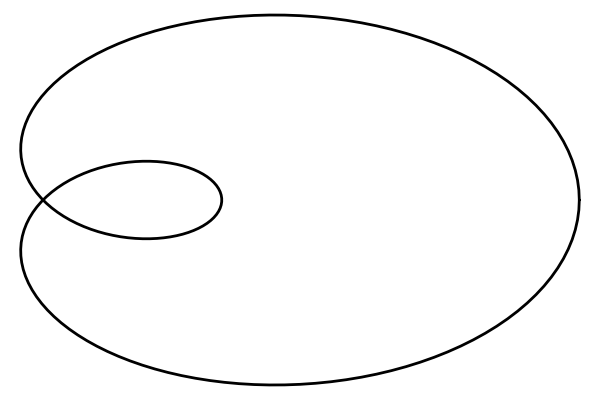
\includegraphics[width=\linewidth]{./assets/3-1-1/limacon-a-gt-1.png}
    \caption{$|a|>1$}
  \end{subfigure}
  \begin{subfigure}[b]{0.3\linewidth}
    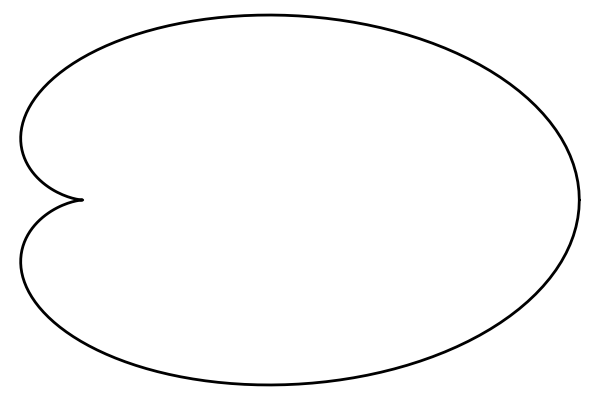
\includegraphics[width=\linewidth]{./assets/3-1-1/limacon-a-eq-1.png}
    \caption{$|a|=1$}
  \end{subfigure}  
  \begin{subfigure}[b]{0.3\linewidth}
    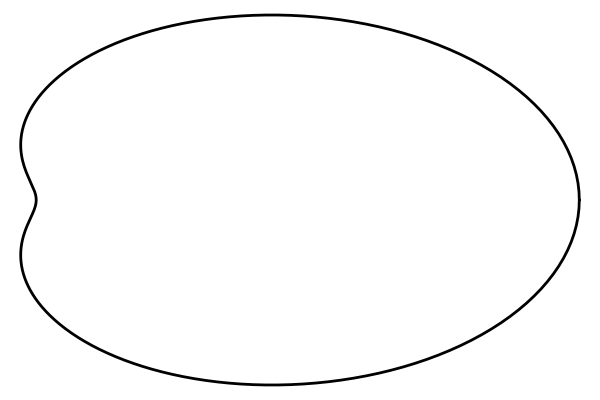
\includegraphics[width=\linewidth]{./assets/3-1-1/limacon-a-lt-1.png}
    \caption{$|a|<1$}
  \end{subfigure}
 
  \caption*{A limaçon (a) will degrade to a cardioid (b).}
\end{figure}
\clearpage
When $|a|>1$, $\gamma$ will have a self intersection. By definition, a simple closed curve is not to have any self-intersections.\\

\noindent
\underline{Proof of self-intersection when $|a|>1$:}\\\\
\indent

For some $t_0, \ t_1 \in [0,T)$, where $\gamma$ is $T$-periodic, $\gamma$ will have the same position twice if $\gamma$ has a self-intersection. Meaning,
$$
\gamma(t_0) \ = \ \gamma(t_1)
$$
but $t_0 \neq t_1$.\\

Solving $\gamma(t_0) = \gamma(t_1)$  for $t_1$ and $t_0$, we will arrive at
$$
t_0 = cos^{-1}\left(-\frac{1}{a}\right)
$$
$$
t_1 = 2\pi - t_0
$$

At $t_0$ and $t_1$, our position will be at the self-intersection and potential cusp of the curve if it were a cardioid; meaning, when $|a| = 1$.\\
This should prove that when $|a|>1$, $\gamma$ cannot be a simple closed curve.\\

\noindent
\underline{$\gamma$'s complement to disjoint sets $Int(\gamma)$ and $Ext(\gamma)$:}\\\\
\indent
When $|a|>1$, $\gamma$ has a self-intersection, and therefore two sets of $Int(\gamma)$, one of which is the subset of the other, as well as a single $Ext(\gamma)$ set.

\begin{figure}[h!]
  \centering
      \begin{subfigure}[b]{0.6\linewidth}
    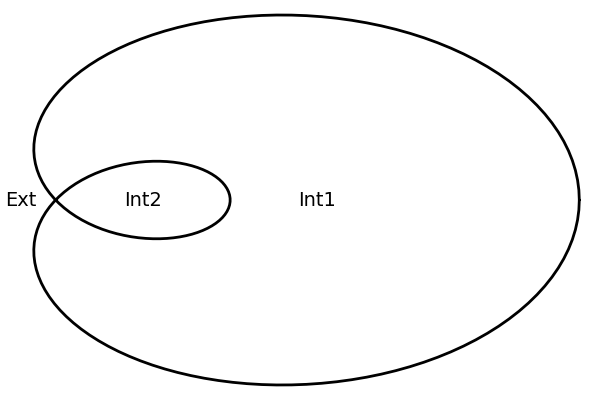
\includegraphics[width=\linewidth]{./assets/3-1-1/limacon-int-ext.png}
    \caption*{$Int_2$ is a subset of $Int_1$.}
  \end{subfigure}
  \end{figure}
  
  We can then classify these sets as follows, starting from the inside of $\gamma$:\\\\
  $$
  Int_2(\gamma) \ = \ \lbrace  \ (x,y) \in \mathbb{R}^2 \ \vert \ (x,y) < \gamma(t) \in [\gamma(t_0),\gamma(t_1)] \ \rbrace
  $$
 $$
  Int_1(\gamma) \ = \ \lbrace  \ (x,y) \in \mathbb{R}^2 \ \vert \ \gamma(t) \in [\gamma(t_0),\gamma(t_1)]<  (x,y) < \gamma(t) \in [\gamma(0),\gamma(t_0)] \cup [\gamma(t_1),\gamma(2\pi)] \ \rbrace
  $$
\end{document}
This is never printed